\documentclass[tikz]{standalone}
\usepackage{amssymb}
\usetikzlibrary{fadings}

\begin{document}

\LARGE % for the fontsize.

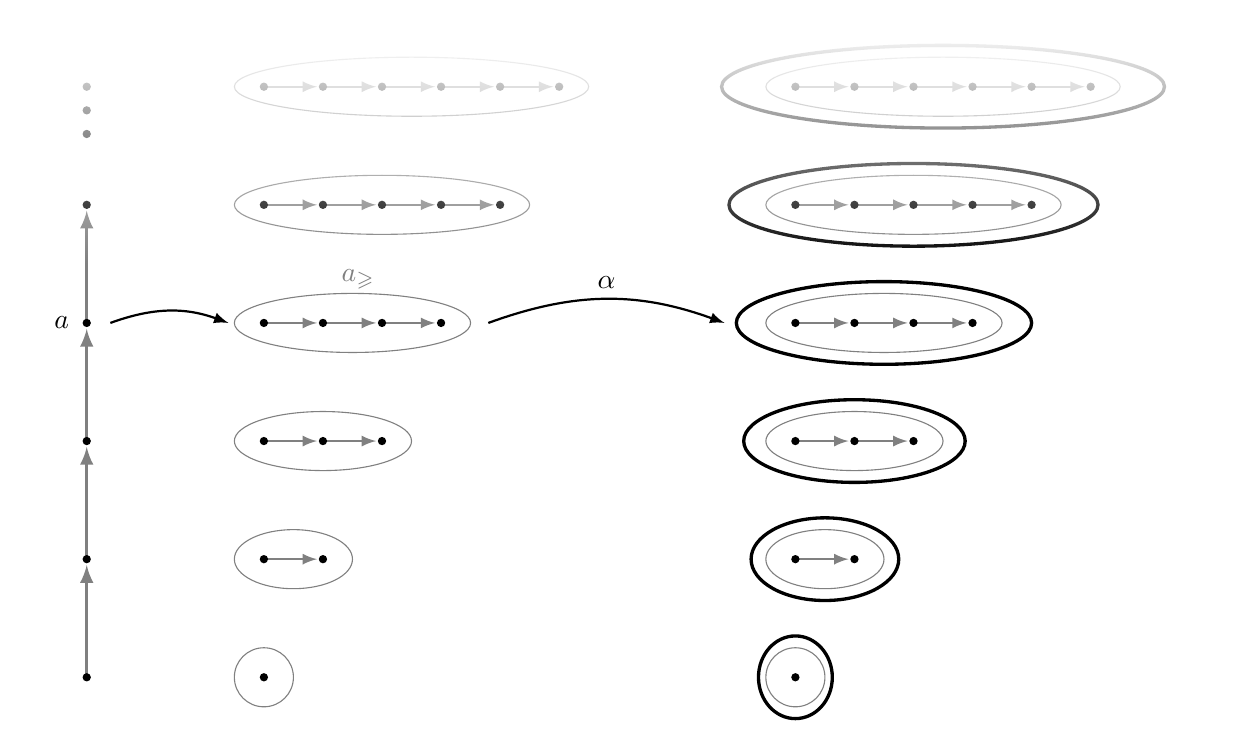
\begin{tikzpicture}[->, >=latex, scale=1.5]

	% === FIRST === (((
	\foreach \n in {0,...,3} \draw [very thick,gray] (0,\n) --++ (0,0.95);
	\foreach \n in {0,...,5} \fill (0,\n) circle (1pt);
	\fill (0,4.8) circle (1pt);
	\fill (0,4.6) circle (1pt);
	% )))

	% === SEC === (((
	\begin{scope}[xshift=1.5cm]
		\foreach \n in {0,...,5} {
			\foreach \m in {0,...,\n} {
				\ifnum\m<\n{\draw [thick,gray] (\m/2,\n) --++ (0.45,0);}\fi
				\fill (\m/2,\n) circle (1pt);
			}
			\draw [gray, shift={(\n/4,\n)}, xscale={(\n+1)/4}]
			(0,0) ellipse (1 cm and 0.25 cm);
		}
	\end{scope}
	% )))

	% === THIRD === (((
	\begin{scope}[xshift=6cm]
		\foreach \n in {0,...,5} {
			\foreach \m in {0,...,\n} {
				\ifnum\m<\n{\draw [thick,gray] (\m/2,\n) --++ (0.45,0);}\fi
				\fill (\m/2,\n) circle (1pt);
			}
			\draw [gray, shift={(\n/4,\n)}, xscale={(\n+1)/4}]
			(0,0) ellipse (1 cm and 0.25 cm);
			\draw [very thick,shift={(\n/4,\n)}, xscale={(\n+1)/4}]
			(0,0) ellipse (1.25 cm and 0.35 cm);
		}
	\end{scope}
	% )))

	% === LABELS AND SHADING === (((
	\node [left=1mm] at (0,3) {\(a\)};
	\draw [thick] (0.2,3) to [out=20 , in=160] ++(1,0);
	\node [gray,above] at (2.3,3.2) {\(a_{\geqslant}\)};
	\draw [thick] (3.4,3) to [out=20 , in=160] node [above] {\(\alpha\)} ++(2,0);
	\fill[path fading=south,color=white!200] (-0.5,5.5) rectangle ++(10,-2);
	% )))

\end{tikzpicture}

\end{document}
